\documentclass[11pt]{article}
\usepackage{graphics}
\usepackage{graphicx} %So we can include .png and .jpg files
\usepackage{url}
\usepackage{verbatim}
\usepackage{fullpage} %Cause it sucks when math runs off the page
\usepackage{makeidx}
\makeindex
%I don't like my paragraphs indented because we have lots of 1-line paragraphs with URLs or code after them
\setlength{\parindent}{0in} 
%I like space between my paragraphs
\setlength{\parskip}{10pt} 


\title{RL-Glue 3.0 Docs}
\author{Adam White}
%\date{}                                           % Activate to display a given date or no date

\begin{document}
\maketitle
\tableofcontents
%\section{}
%\subsection{}


\section{Introduction}
\subsection{Purpose of Document}
This document has been laid out so that it can be used for: 
\begin{enumerate}
\item  {\bf RL-Glue what?} learning about RL-Glue at an abstract level
\item {\bf Compatibility:} making existing C/C++ agents and environments work with RL-Glue
\item {\bf Plugging agents and environments together:} how to write an experiment programs
\item{\bf What function do I use to:} quick function reference for RL-Glue
\end{enumerate}

Recently (September 08) the RL-Glue Project has been split into the RL-Glue Project and RL-Glue Extensions Project. The RL-Glue Project now only includes the RL-Glue interface and plugs for C/C++ agents, environments and experiment programs. The RL-Glue Extensions Project contains codecs for Java, Python and Matlab. The Extensions Project contains the multi-language support code that used to be part of RL-Glue. This document contains {\bf NO} technical details for writing programs: everything is abstracted. See the RL-Glue Technical Documentation distributed with RL-Glue and codec documentation for language specific details on how to implement agents, environments and experiment programs in C/C++, Java, Python and Matlab.
 
\subsection{How to Use This Document}

This document as been subdivided to reflect the five purposed described above. To learn about the major components of RL-Glue and a description of how those components interact see Section \ref{RL-Glue}. To learn how to make an environment and agent programs compatible with RL-Glue we recommend sections \ref{envp1} and \ref{agentp1}. Sections \ref{envp1} and \ref{agentp1} describe only the mandatory functions that RL-Glue environments and agents must implement. Sections \ref{envp2} and \ref{agentp2} describe optional environment and agent functions. To learn about experiment programs and how they interact with RL-Glue see Section \ref{exp}. For quick function reference see Section \ref{ref}.

Frequently asked questions and glossary can be found in sections \ref{faq} and \ref{glos}.

This document and the RL-Glue Project using naming conventions and definitions from Sutton and Barto's ``Reinforcement Learning: An Introduction". We recommend that you review Sutton and Barto to get the most out of the RL-Glue documentation. An online version of Sutton and Barto can be founf here: \url{http://www.cs.ualberta.ca/~sutton/book/the-book.html}.



 
 
\section{RL-Glue Concepts}
\label{RL-Glue}
A large part of studying and researching reinforcement learning is experimentation. When writing an agent, ensuring it makes exploratory moves to discover the world is important to achieving an optimal policy. It is similarly important that experimenters are easily able to "explore" new algorithms and ideas without the prohibitive cost of writing the necesary experimentation code. One of the functions of RL-Glue is to simplify and speed up the process of writing an experiment so that every idea can be tested. 


Another important part of learning is evaluation and improvement. With agents, learning is often a cycle of policy and representation evaluation and improvement.  An agent will roam the world and gain more information about the states it encounters. The agent then uses this new data to evaluate how accurate the value function was and adjusts its behaviour (policy) based on the new value function. Similiarily, in research and development it is important to look at other work being done in the field, compare your own performance and then improve. One goal for RL-Glue is to provide a consistent tool for running and comparing varied agents and environments from diverse sources. A common problem for reinforcement learning researchers arrises when an experimenter wishes to compare their own work with previously established results. Pre-RL-Glue, the solution was often to reverse engineer code for the experiment based on the results and environment/agent descriptions provided in papers.  When an author provided their own source, there was still the issue of deciphering the original code and piecing in a new agent or environment. With RL-Glue, an author can make the necessary RL-Glue agent/environment/experiment programs  available to the public such that another author can rerun the original experiment and easily plug in their own code to compare performance.  Competitions for agents using RL-Glue have been run at NIPS and ICML in recent years, further exemplifying the utility of RL-Glue to the research community.
 
\begin{figure}
\label{fig1}
\begin{center}
%\htmlimage{scale=0.5}
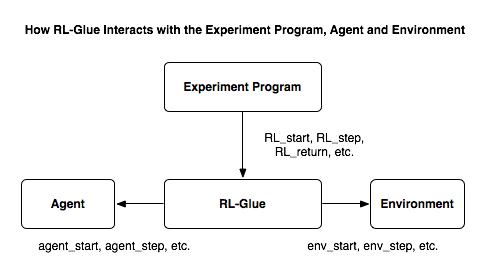
\includegraphics[height=60mm]{images/glue_connections_no_shadow.png}
\caption{The RL-Glue Standard. Arrows indicate function call direction.}
\end{center}
\end{figure}

RL-Glue is both a set of ideas and standards, as well as a software implementation. In theory, RL-Glue is a protocol for all RL researchers to follow. Having this very simple standard of necessary functions facilitates the exchange and comparison of agents and environments without limiting their abilities. As software, RL-Glue is functionally a test harness to "plug in" agents, environments and experiment programs (previously titled benchmarks) without having to continually rewrite the connecting code for these pieces. An experiment program is some very simple code stating how many times to run an agent in an environment and what data should be extracted from the agent and environment. Provided the agent, environment, and experiment program follow the RL-Glue protocol by implementing the few necessary functions, they can easily be plugged in with the RL-Glue code to have an experiment running quite effortlessly. Figure \ref{fig1} is a diagram which shows how function calls work in RL-Glue.



The Experiment Program contains the "main function" which will then make all of it's requests for information through RL-Glue. These requests are usually related to setting up, starting and running the experiment and then gathering data about the agent's performance. The experiment program should never have access to the agent or environment directly, all contact should always go through the RL-Glue interface first.  There is also no direct contact between the agent and the environment. Any information the agent or environment returns is passed through RL-Glue to the module which needs it.  



\subsection{Agents, Environments and Experiment Programs}
Understanding agents and environments is a fundamental part of understanding reinforcement learning. A more detailed explanation of reinforcement learning, and its definitions for agents and environments, can be obtained from Reinforcement Learning: An Introduction (Sutton, Barto. 1998).  The agent, when distilled to basics, is both the learning algorithm and the decision maker. For RL-Glue's purpose, the agent only needs to decide which action to take at every step. The environment should store all the relevant details of the world of your experiment. This should include knowledge of the current state representation (the observation) as well as some method for determining state transitions and rewards. When writing code for an experiment, RL-Glue has been structured to place separation between the agent and environment. This division of the agent and environment both helps create modularized code and is theoretically desirable.


The experiment program is familiar to anyone who has written code to run an reinforcement learning experiment on their own. Akin to the typical main function in many reinforcement learning experiments, an RL-Glue experiment program is a control loop which runs the agent through the environment {\bf x} number of times, perhaps doing {\bf y} trials of these {\bf x} episodes, all the while gathering data about how efficiently the agent has behaved or how quickly it has learned. RL-Glue provides several functions (Section \ref{ref}) to assist in writing an experiment program.


When writing an agent , environment or experiment program for RL-Glue it is necessary to adhere to the interfaces (the RL-Glue Protocol) set out in Section \ref{ref}. 

\section{RL-Glue Environment Programs}
\label{env}
The environment represents everything outside the agents direct control. In a gridworld, the environment is the grid, including obstacles, rewards, start states, termination conditions and transition function. In a robotic task, the environment would also include the robot's body, as the robot as the robot does not have complete, deterministic control over its motors. The environment is basically everything that is not the agent.

In RL-Glue, the environment is defined by a set of parameterized functions that the RL-Glue interface queries on behalf of the experiment program. These functions define what the environment does before an experiment begins, at the beginning of an episode, on every remaining step of an episode and after the experiment is completed. The following sections describe the basic requirements of an RL-Glue environment, a complete list of all environment functions and specific details on how to implement the environment functions in C and C++.


\subsection{Essential Components Of A RL-Glue Environment}
\label{envp1}

Every RL-Glue environment must define and initialize the action and observation types (rewards are always real-valued scalars) and define the env\_start and env\_step functions.   

\subsubsection{Observation and Action Encoding}
The representation of the observation and the action must be one of the following: 
\begin{itemize}
\item an integer
\item a double
\item a character
\item array of integers
\item array of doubles
\item array of characters
\end{itemize}
Although this seems restrictive, in practice it should be easy to represent many observation and action types in this format. In a gridworld, for example, the action can be a single integer with values 0-3 (for N,S,E,W) and the observation can also be an integer for the agent's grid position (which is also the state of the environment, in this case). In Mountain Car, the actions are discrete (0-2) and the observation is the cars position and velocity (both real numbers). The action can be represented with and integer and the observation can be a two dimensional double array. 


Details on how to encode observation and action types in C and C++ is described in the ``RL-Glue Technical Documentation" included the project source.

\subsubsection{Environment Start}
Writing env\_start is very simple. The function takes no input and simply returns an observation. The env\_start function signifies the beginning of an episode; env\_start chooses the initial state of the environment and returns the corresponding observation. For example, the following pseudo code selects a random start state for a grid world and returns the observation:
\begin{tabbing}
1. {\bf env\_start}\= $\rightarrow$ observation\\
2. \>state = rand()*num\_states\\
3. \>set observation equal to state\\
4. {\bf return} observation
\end{tabbing}
The RL-Glue Technical Documentation describes how to implement line 3 in C/C++.

\subsubsection{Environment Step}
The final essential piece of an RL-Glue environment is the env\_step function. The env\_step function must take an action as input and produce a observation, reward and a termination flag as output. In most RL problems the  env\_step function updates the internal state of the environment, tests for end of episode and returns the new observation of state and current reward. In other words, step function encodes the state transition and reward functions. Keeping with the grid world example, the following step function would be a valid env\_step function:
\begin{tabbing}
1. {\bf env\_step}\=(Action a) $\rightarrow$ reward, observation, flag \\
2. \>newState = updateState(a, oldState)\\
3. \> flag = isTerminal()\\
3. \> reward = -1\\
4. \>set observation equal to newState\\
5. \>oldState = newState\\
6. {\bf return} reward, observation, flag
\end{tabbing}
Here we assume the existence of a state update function and an isTerminal function that checks if the current state is a terminal state.

So thats it. Just define the types of actions and observations and write two functions and you have a valid RL-Glue compatible environment. In later sections we will go over advanced environment functions and describe the syntactic details of actually coding an environment in C and C++. 

\subsection{Additional Components Of A RL-Glue Environment}
\label{envp2}

So far we have only scratched the surface of what kinds of environments you can write in RL-Glue. Additional environment function can be written to initialize data structures, get and set the state of the environment, get and set the random seed and send generic string messages to the environment. Before we go on describing these functions it is useful to understand the task specification language that is used in RL-Glue to encode basic information about environments. 

\subsubsection{Task Specification Language}
\label{task}
In an effort to provide the agent writer with simple and concise information about the environment a Task\_specification is passed from the environment, through the interface, to the agent. The environment's init method (env\_init) encodes information about the problem in a ASCII string. The string is then passed to the agent's init method (agent\_init).  This information can also be used to check that the agent and environment are suitable for each other. A few example Task\_specifications are provided below.
\\\\
The agent is responsible for parsing any relevant information out of the Task\_specification in the init method. A generic Task\_specification parsing function is provided with RL-Glue 2.0 for all C/C++ users. This simple parser will return a structure containing the information encoded in the Task\_specification, such as the Observation and Action dimensions, arrays of Observation and Action variable ranges, and arrays of Observation and Action variable types. More information about the parser and the parsed task spec struct can be found here.
\\\\
The Task\_specification is stored as a string with the following format:
\begin{verbatim}
     "V:E:O:A:R"
\end{verbatim}		
For example, this is a sample task\_specification provided as one of the examples below:
\begin{verbatim}
     "2:e:1_[i]_[0,N-1]:1_[i]_[0,3]:[-1,0]"
\end{verbatim}     
The V corresponds to the version number of the task specification language. E corresponds to the type of task being solved. It has a character value of 'e' if the task is episodic and 'c' if the task is continuing. O and A correspond to Observation and Action information respectively. Finally, the R corresponds to the range of rewards for the task. Within each of O, A and R a range can be provided, however if the values are unknown or infinite in magnitude, two special input values have been defined.
\\\\
The format of O and A are identical. We will describe the form of O only. O contains three components, separated by underscore characters ("\_") :
\begin{verbatim}        
     #dimensions_dimensionTypes_dimensionRanges
\end{verbatim}
\#dimensions is an integer value specifying the number of dimensions in the Observation space. dimensionTypes is a list specifying the type of each dimension variable. The dimensionTypes list is composed of \#dimensions components separated by comma characters (``,") within square brackets ([x1,x2,x3,..., xn] where xi  represents the ith value). Each comma-separated value in the list describes the type of values assigned to each Observation variable in the environment. In general, Observation variables can have one of the following 2 types:
\begin{verbatim}
     `i' - integer value
     `f' - float value
\end{verbatim}
Thus a dimensionTypes list corresponding to an Observation space with 1 dimension has the following form:
\begin{verbatim}
     [a] where a is an element of [`i',`f']
\end{verbatim}
So a dimensionTypes list with one integer value would be:    
\begin{verbatim}    
     [i]
\end{verbatim}     
An Observation space with 2 dimensions would have a dimensionTypes with the following form:
\begin{verbatim}
     [a,b] where a and b are elements of [`i',`f']
\end{verbatim}
indicating the value type of the first (a) and second (b) Observation variables. Thus a three dimensional Observation with one float, integer dimension and another float dimension would have the following dimensionTypes:
\begin{verbatim}
     "[f,i,f]"
\end{verbatim}
The dimensionRanges is a list specifying the range of each dimension variable in the Observation space.  The dimensionRanges is composed of \#dimensions components separated by underscore characters. Each dimensionRanges component specifies the upper and lower bound of values for each Observation variable. If the bounds are unknown or unspecified, you can leave an empty space in the place of a value. If the bounds are positive or negative infinity, you can use inf or -inf to represent your range. These can be used in combination. For example one valid range could be an unknown lower bound and infinite upper bound, or a lower bound of -inf and an upper bound of 1. You can be as precise (though you must be accurate) as you wish. A dimensionRanges corresponding to an Observation space with a single dimension variable would have the following form:
\begin{verbatim}
     [O1MIN, O1MAX]
\end{verbatim}
So a dimensionRanges list for binary dimension varaible would be: [0,1]
A dimensionRanges list for variable with no upper or lower bound unspecified would be: [] or [,] (both are valid).
A dimensionRanges with one or two unbounded value can take on a value of inf or -inf. Eg [0, inf] or [-inf,1] or [-inf,inf].
\\\\
An Observation space with 2 dimensions would have a dimensionRanges with the following form:
\begin{verbatim}
     [O1MIN, O1MAX]_[O2MIN, O2MAX]
\end{verbatim}
indicating the minimal and maximal values of Observation variables O1 and O2 respectively. This definition can be then trivially extended to Observation spaces with N dimensions.
\\\\
NOTE: the dimensionRanges of an Observation space with 1 or more unbounded values may not be representable in this way. An unbounded value has no minimal or maximal range. Thus, we simply do not specify the range in the dimensionRanges for any Observation variables with unbounded values. For example, consider a problem with 3 Observation dimensions. The first and third Observation variables have interval values and the second has unbounded ratio value. The corresponding dimensionRanges for this problem is encoded as:
\begin{verbatim}
     [O1MIN, O1MAX]_[,]_[O3MIN, O3MAX]
\end{verbatim}
indicating the minimal and maximal values of Observation variables O1 and O3.
\\\\
The format of A (Action space information) is identical to that of O (Observation space information) and thus the definitions above hold for Action spaces.
\\\\
Lastly the R (Reward space information) is merely a range specifier. By the Reward Hypothesis there is only ever one reward signal (which in RL-Glue is always a floating point number) so the \#dimensions and dimensionType information becomes meaningless. The reward range can again be specified to be unknown or infinite in the same manner as the Observation ranges.  A rewardRange follows the following form:
\begin{verbatim}
     [rewardMin, rewardMax]
\end{verbatim}
In the case of a reward with rewards -1 or 0 the rewardRange would appear as such: [-1,0].
If no lower bound was known and the upper bound was positive infinity, the rewardRange would appear as such: [,-inf]
\subsubsection{Example Task\_Specification}
Consider a simple gridworld with Actions North, South, East and West and a single dimension Observation of grid position. If we encode actions as 0, 1 ,2 ,3 and position as an integer between 0 and N-1, we get the following Task\_specification:
\begin{verbatim}
     "2:e:1_[i]_[0,N-1]:1_[i]_[0,3]:[-1,0] "
\end{verbatim}
This Task\_specification provides the following information:
\begin{description}
\setlength{\itemsep}{-1mm}
\item[-] RL-Glue version 2.0 supported
\item[-] the task is episodic
\item[-] Observation space has one dimension
\item[-] the Observation variable has integer values (discrete state)
\item[-] range of Observation variable is 0 to N-1
\item[-] Action space has one dimension
\item[-] the Action variable has integer values (discrete actions: tabular)
\item[-] range of Action variable is 0 to 3
\item[-] range of the rewards is -1 to 0
\end{description}


        
\subsubsection{Environment initialization and Cleanup}        
Most environments need to store an internal state representation  and therefore many environment programs you write will need to allocate and deallocate data structures before and after a learning experiment. The env\_init function allocates any global data structures and variables that will be accessed by the start and step functions. For example, the env\_init method might initialize the tabular state variable to zero and allocate a {\it numStates X numStates} state transition array. The env\_init function can optionally define a Task Specification string. The env\_init function must return a string, but it can return NULL or an empty string if the Task Specification is not required for your experiment. The Task Specification is described in detail in the previous section (Section \ref{task}).


The env\_cleanup function usually deallocates or frees anything allocated in env\_init.

\subsubsection{Environment Message}
Once in a while you will find yourself wishing there was an environment function that was part of RL-Glue. The env\_message function allows you to exactly this: you can send a string message to the environment and it can respond with a string. For example to disable random starting states:
\begin{tabbing}
1. env\_\=message(inMessage) $\rightarrow$ outMessage\\
2.\> {\bf if} in\=Message == ``turnOffRandomStarts"  \\
3. \>\> randStarts = false\\
4. \> {\bf end} \\
5. {\bf return} ``1"
\end{tabbing}

\subsubsection{Environment Get and Set Sate}
It is often necessary to record the state of the environment and then reset the environment to a particular state to evaluate learning performance. For example, one might want to repeatedly evaluate the performance of a stochastic policy starting from a finite set of interesting states. The env\_get\_state\_key function returns a state\_key that can be used to restore the environment to the current state when the key was created. The state\_key is the same data type as the observations and actions; the state\_key must be an int, double, character, int array, double array or character array. The env\_set\_state takes a state\_key as input and simply restores the environment to the state encoded in the key. The state\_key can be as simple as a integer state label, in the case of a gridworld, or a some function of an array, in the case of a simulated robot navigation task. 

The get and set state functions are meant to be used during a single learning experiments not across runs. For example, the following experiment is valid:
\begin{tabbing}
1. initialize RL-Glue\\
2. {\bf until} observation ``cliff" {\bf do} next step of episode\\
3. get state key form environment and store in stateKey\\
4. {\bf for} \=100 steps\\
5. \> set environment state to stateKey\\
6. \> run an episode
\end{tabbing}
Storing a state key in a file and then using that state key in a different experiment program or later time is outside the intended usage of the env\_get\_state and env\_set\_state functions. It might work with some RL-Glue environments and not others.
        
\subsubsection{Environment Get and Set Random Seed}
It can be useful to record and set the seed of the random number generator. Although the random seed can be well thought of as part of the state of the environment there may be times when it is more convenient access the random seed only with env\_get\_random\_seed and env\_set\_random\_seed functions. The environment get and set random functions return and take as input a random\_seed\_key, like the state\_key for setting states. 

Like the get and set state functions, env\_get\_random\_seed and env\_set\_random\_seed functions should not be used to store and set the random seed between distinct runs of RL-Glue.

A compete list of environment functions can be found in Section \ref{Eref}.










\section{RL-Glue Agent Programs}
\label{agent}
An RL-Glue agent can be as simple as a program the returns a random number between one and zero on every step or a more advanced algorithm that learns a model of the reward and transition functions of environment while maximizing reward. The agent program is a decision maker first and foremost: it must return an action when queried by RL-Glue. Many Rl-Glue agents, however, learn the best action to pick by learning from the sequence of observations, actions and rewards during an episode. Agent programs, like environments, are completely defined by a set of functions you must implement. Rl-Glue calls these agent functions during an experiment, as directed by the experiment program. Whether you are writing a random agent or a learning agent you usually need only implement a few functions. This section covers the basic requirements of an RL-Glue agent, describes a number of optional agent functions and describes how to implement these agent functions in C and C++.
\subsection{Essential Components Of A RL-Glue Agent}
\label{agentp1}

An agent program is fully compatible with RL-Glue if it implements three functions: agent\_start, agent\_step and agent\_end. 

\subsubsection{Action Types}
The three agent functions take observations and rewards as input and return actions. The observations and rewards are created by the environment, so the agent program needs to only read their values. The actions, however, must be defined by the agent.

\subsubsection{Agent Start}
The agent\_start function selects the first action at the beginning of an episode based on the first observation of the environment. The agent\_start function does not receive a reward as input; agent\_start usually contains no learning update code. For example, the following function selects the first action based on the current value function estimate:
\begin{tabbing}
1. age\=nt\_start (observation) $\rightarrow$ action\\
2. \> {\bf for} \= each action {\it i}\\
3.\>\> {\bf if} highest valued action ( Q(observation,{\it i}) )\\ 
4. \>\>{\bf then} store {\it i} as maxAction\\
5. \> {\bf set} action equal to newAction\\
6. {\bf return} action
\end{tabbing}
The following sections will describe how to perform step 5 in several different programming languages.

\subsubsection{Agent Step}
The agent\_step function encodes the heart of the agents' learning algorithm and action selection mechanism. At a minimum the step function must return an action every time it is called. In most learning agents, the step function queries the agent programs action selection function and performs a learning update based on the input observation and reward. The following agent\_step function does a SARSA update on a tabular value function Q:
\begin{tabbing}
1. age\=nt\_step(reward, observation) $\rightarrow$ action\\
2. \>newAction = egreedy(observation)\\
3. \> QofOld = Q(oldState,oldAction)\\
4. \> QofNew = Q(observation,newAction) \\
5. \> Q(oldState,oldAction) = QofOld + $\alpha$[reward + $\gamma$QofNew - QofOld]\\
6. \> oldState = observation\\
7.\> oldAction = newAction\\
8. \> {\bf set} action equal to newAction\\
9. {\bf return} action
\end{tabbing}  
Notice that the agent program must explicitly store the observation and action from the previous time step. RL-Glue does not make the history of actions, observations and rewards available to the agent or environment.

\subsubsection{Agent End}
In episode task the environment enters a terminal state that ends the episode. RL-Glue responds to the end of an episode by calling the agent\_end function; passing the reward produced on the last transition to the agent and signaling the end of the current episode. The agent\_end function usually performs a final learning update based on the last transition and any other end-of-episode routines, such as clearing eligibility traces. If the environment is non-episodic RL-Glue will not query agent\_end.

The agent\_end function does not receive the final observation from the environment. In many learning problems this is of no consequence because the agent does not make a decision in the terminal state. If, however, the agent were learning a model of the environment, information about the final transition would be important. In this case, it is recommended that the environment be augmented with a terminal state that has a reward of zero on the transition into it. This choice was made to keep the RL-Glue interface as minimal and light-weight as possible. 

\subsection{Additional Components Of A RL-Glue Agent}
\label{agentp2}

\subsubsection{Agent Initialization and Cleanup}
Agent programs, like environments, often need to allocate and free various data structures. The agent\_init and agent\_cleanup function do not take any input or return an data and are called at the beginning and end of a learning experiment, respectively. The agent\_init function also receives the Task Specification string as input. The agent\_init function usually parses the Task Specification and stores various information encoded in the string. For example, after parsing the Task Specification, the agent\_init function can then initialize the value function array to the size state space using the number of states from the Task Specification. Remember the Task Specification is not required to contain any information (NULL or empty string). The RL-Glue codecs provide parsers that return a structure/object given a Task Specification string.     

\subsubsection{Agent Message}
The agent\_message function isused to send an arbitrary string message to the agent program. This function can be used to change agent parameters, notify the agent that the exploration phase is over, and request the name of the agent program, for example.



\section{RL-Glue Experiment Programs}
\label{exp}
Usually the shortest and easiest part of writing your first learning experiment is writing the experiment program. The experiment program has no interface to implement and is mostly comprised of calls to the already existing RL-Glue functions. The experiment program has four main duties: a) start the experiment b) specify how many times to run the experiment c) extract data and possibly analyze d) end the experiment and clean up.  One thing to note is that it is only the RL-Glue interface functions available to the experiment program. No agent or environment implemented functions should be directly accessed by the experiment program.

\subsection{Basic Experiment Programs}
\label{expp1}

At a minimum the experiment program must call RL\_init and RL\_cleanup and execute several time steps of agent-environment interaction. The following pseudo code represents a simple experiment program.
\begin{tabbing}
1. RL\_init()\\
2. RL\_start()\\
3. steps=0\\  
4. terminal=false \\
5. {\bf while} \=steps $<$ 100 {\bf and not} terminal\\
6.\> terminal,reward,observation,action = RL\_step()\\
7. RL\_cleanup()
\end{tabbing}
This experiment program initializes the agent and environment (RL\_init), calls the start functions of the agent and environment (RL\_start) and then executes a 100 or less step episode. 

The RL\_step function calls the env\_step function passing it the most recent agent action (in this case from agent\_start). The env\_step function returns the new observation, reward and terminal flag. If the flag {\bf is not} set the agent\_step function is called with the new observation and reward as input arguments. The action returned by agent\_step is stored by RL-Glue until the next call to RL\_step. If the flag {\bf is} set, the agent\_end function is called with the reward as input. This process continues until either the flag is set or 100 steps are completed. 

Using the RL\_step function gives the experiment program designer access to all the data produced during an episode; however, it is often more convient to use the RL\_episode function when step-level control is not needed. Lines 5 and 6, in the above experiment program, can be replaced by a single call to RL\_episode(100). If the input to RL\_episode is zero, control will return to the experiment program if and only if the environment enters a terminal state.

The RL\_step function allows the experiment program to record/sum/average the reward, but the RL\_episode function returns no values. The RL\_return and RL\_num\_steps functions allow the experiment program to obtain reward and number of steps taken. Specifically, RL\_return returns the sum of rewards accumulated during the current or most recently completed episode. The RL\_num\_steps returns the number of steps elapsed during the current or most recently completed episode. 

Putting these new functions together we can write a more useful experiment program:
\begin{tabbing}
1. RL\_init()\\
2. theReturn = 0\\
3. {\bf for} \= 1 = 1:100\\
4. \> RL\_episode(1000)\\
5. \> theReturn += RL\_return()\\
6.  {\bf Print} theReturn/100\\
7. RL\_cleanup()
\end{tabbing}
The above experiment program runs 100 episodes, each with max length 1000, and computes the average cumulative reward per episode.
\subsection{Advanced Experiment Programs}
\label{expp2}


As you know from previous sections (about agent and environment programs) there are several optional agent and environment functions that provide more advanced control. These functions are access through calls to the RL-Glue interface from an experiment program. For example, to send a message to the agent use RL\_agent\_message. To get the state key from the environment use RL\_get\_state. The pattern is simple to follow:
\begin{itemize}
\item RL\_set\_state() $\rightarrow$ env\_set\_state()
\item RL\_get\_random\_seed() $\rightarrow$ env\_get\_random\_seed()
\item RL\_set\_random\_seed() $\rightarrow$ env\_set\_random\_seed()
\item RL\_env\_message() $\rightarrow$ env\_message

\end{itemize}
We can now produce more advanced experiment programs that would be used in reinforcement learning research:
\begin{tabbing}
1. RL\_init()\\
2. numSteps = 0\\
3. {\bf for} \= 1 = 1:1000\\
4. \> RL\_episode(1000)\\
5. RL\_agent\_message("freezeAgentPolicy")\\
6. {\bf for} \= 1 = 1:100\\
7. \> RL\_episode(1000)\\
8. \> numSteps += RL\_num\_steps()\\
9.  {\bf Print} numSteps/100\\
10. RL\_cleanup()
\end{tabbing}





\section{Command and Function Reference}
\label{ref}
Once your comfortable with the basics and you have written a few agents and environment you may often find yourself wondering "I need to do {\bf X} what function should I use". You may also wonder what is the "intended purpose" of a particular RL-Glue function, when you are reviewing someone else's agent or environment code. This section provides a complete listing of all agent, environment and RL-Glue interface function for quick reference.
\subsection{Agent Functions}
 
Every agent must define all of the following routines. Note these functions are only accessed by the RL-Glue. Experiment programs should not try to bypass the Glue and directly access these functions.
\\\\
agent\_start:  agent\_start(first\_observation) $\rightarrow$ first\_action\\
Given the first\_observation (the observation of the agent in the start state) the agent must then return the action it wishes to perform. This is called once if the task is continuing, else it happens at the beginning of each episode.
\\\\
agent\_step: agent\_step( reward, observation) $\rightarrow$ action\\
This is the most important function of the agent. Given the reward garnered by the agent's previous action, and the resulting observation, choose the next action to take. Any learning (policy improvement) should be done through this function.
\\\\
agent\_end: agent\_end(reward)\\
If the agent is in an episodic environment, this function will be called after the terminal state is entered. This allows for any final learning updates. If the episode is terminated prematurely (ie a benchmark cutoff before entering a terminal state) agent\_end is NOT called.
\\\\
agent\_init: agent\_init(task\_specification)\\
This function will be called first, even before agent\_start. The task\_specification is a description of important experiment information, including but not exclusive to a description of the state and action space. The RL-Glue standard for writing task\_specification strings is found here.  In agent\_init, information about the environment is extracted from the task\_specification and then used to set up any necessary resources (for example, initialize the value function to a prelearning state).
\\\\
agent\_cleanup: agent\_cleanup()\\
This function is called at the end of a run/trial and can be used to free any resources which may have allocated in agent\_init. Calls to agent\_cleanup should be in a one to one ratio with the calls to agent\_init.
\\\\
agent\_freeze: agent\_freeze()\\
Signals to the agent that training has ended. Requests that the agent freeze its current policy and value function (ie: stops learning and exploration).
\\\\
agent\_message:agent\_message(input\_message) $\rightarrow$ output\_message\\
The agent\_message function is a jack of all trades and master of none. Having no particular functionality, it is up to the user to determine what agent\_message should implement. If there is any information which needs to be passed in or out of the agent, this message should do it. For example, if it is desirable that an agent's learning parameters be tweaked mid experiment, the author could establish an input string that triggers this action. Likewise, if the author wished to extract a representation of the value function, they could establish an input string which would cause agent\_message to return the desired information.
                          
\subsection{Environment Functions}
\label{Eref}
Every environment must define all of the following routines. Note these functions are only accessed by the RL-Glue. Experiment programs should not try to bypass the Glue and directly access these functions.
\\\\
env\_start: env\_start() $\rightarrow$ first\_observation\\
For a continuing task this is done once. For an episodic task, this is done at the beginning of each episode. Env\_start assembles a first\_observation given the agent is in the start state. Note the start state cannot also be a terminal state.
\\\\
env\_step: env\_step(action) $\rightarrow$ reward, observation, terminal\\
Complete one step in the environment. Take the action passed in and determine what the reward and next state are for that transition.
\\\\
env\_init: env\_init() $\rightarrow$ task\_specification\\
This routine will be called exactly once for each trial/run. This function is an ideal place to initialize all environment information and allocate any resources required to represent the environment. It must return a task\_specification which adheres to the task specification language. A task\_specification stores information regarding the observation and action space, as well as whether the task is episodic or continuous.
\\\\   
env\_get\_state: env\_get\_state() $\rightarrow$ state\_key\\
The state\_key is a compact representation of the current state of the environment such that at any point in the future, provided with the state\_key, the environment could return to thatstate. Note that this does not include the agent's value function, it is merely restoring the details of the environment. For example, in a static grid world this would be as simple as the position of the agent.
\\\\
env\_set\_state: env\_set\_state(state\_key)\\
Given the state\_key, the environment should return to it's exact formation when the state\_key was obtained. 
\\\\
env\_get\_random\_seed: env\_get\_random\_seed() $\rightarrow$ random\_seed\_key\\
Saves the random seed object used by the environment such that it can be restored upon presentation of random\_seed\_key.
\\\\
env\_set\_random\_seed: env\_set\_random\_seed(random\_seed\_key)\\
Sets the random seed used by the environment. Typically it is advantageous for the experiment program to control the randomness of the environment. Env\_set\_random\_seed can be used in conjunction with env\_set state to save and restore a random\_seed such that the environment will behave exactly the same way it has previously when it was in this state and given the same actions.
\\\\                       
env\_cleanup: env\_cleanup()\\
This can be used to release any allocated resources. It will be called once for every call to env\_init.
\\\\
env\_message:env\_message(input\_string) $\rightarrow$ output\_string\\
Similar to agent\_message, this function allows for any message passing to the environment required by the experiment program. This may be used to modify the environment mid experiment. Any information that needs to passed in or out of the environment can be handled by this function.


\subsection{Interface Routines Provided by the RL-Glue}

The following built in RL-Glue functions are provided primarily for the use of the experiment program writers. Using these functions, the experiment program gains access to the corresponding environment and agent functions. The implementation of these routines are to be standard across all RL-Glue users. To ensure agents/environments/experiment programs can be exchanged between authors with no changes necessary, users should not change the RL-Glue interface code provided.
\\\\      
To understand the following, it is helpful to think of an episode as consisting of sequences of observations, actions, and rewards that are indexed by time-step as follows:

o0, a0,  r1, o1, a1,  r2, o2, a2, ..., rT, terminal\_observation
\\\\
where the episode lasts T time steps (T may be infinite) and terminal\_observation is a special, designated observation signaling the end of the episode.
\begin{tabbing}
RL\_\=init() \\
\>agent\_init(env\_init())
\end{tabbing}
This initializes everything, passing the environment's task\_specification to the agent. This should be called at the beginning of every trial.
\begin{tabbing}
RL\_\=start() $\rightarrow$ o0, a0\\
\>global upcoming\_action\\
\>o = env\_start()\\
\>a = agent\_start(o)\\
\>upcoming\_action = a\\
return o,a
\end{tabbing}

Do the first step of a run or episode.  The action is saved in upcoming\_action so that it can be used on the next step.
\begin{tabbing}
RL\_\=step() $\rightarrow$ rt, ot, terminal, at\\
\>global upcoming\_action\\
\>r,o,terminal = env\_step(upcoming\_action)\\
\>if ter\=minal == true\\
\>\>    agent\_end(r)\\
\>\>    return r, o,terminal\\
\>else\=\\
\>\>    a = agent\_step(r, o)\\
\>\>    upcoming\_action = a\\
\>return r, o, terminal, a
\end{tabbing}
Take one step.  RL\_step uses the saved action and saves the returned action for the next step.  The action returned from one call must be used in the next, so it is better to handle this implicitly so that the user doesn't have to keep track of the action.  If the end-of-episode observation occurs, then no action is returned.
\begin{tabbing}     
RL\_\=episode(steps)\\
\>num\_steps = 0\\
\>o, a = RL\_start()\\
\>num\_steps = num\_steps + 1\\
\>list = [o, a]\\
\>while\=  \ o $\neq$ terminal\_observation\\
\>\>    if(st\=eps $\neq$ 0 and num\_steps $\geq$ steps)\\
\>\>\>    end\\
\>\>    els\=e\\
\>\>\>    r, o, a = RL\_step()\\
\>\>\>    list = list + [r, o, a]\\
\>\>\>    num\_steps = num\_steps + 1\\
\>                agent\_end(r)\\
\end{tabbing}
Do one episode until a termination observation occurs or until steps steps have elapsed, whichever comes first.  As you might imagine, this is done by calling RL\_start, then RL\_step until the terminal observation occurs.  If steps is set to 0, it is taken to be the case where there is no limitation on the number of steps taken and RL\_episode will continue until a termination observation occurs. If no terminal observation is reached before num\_steps is reached, the agent does not call agent\_end, it simply stops.
\\\\
RL\_return() $\rightarrow$ return
\\\\
Return the cumulative total reward of the current or just completed episode.  The collection of all the rewards received in an episode (the return) is done within RL\_return however, any discounting of rewards must be done inside the environment or agent.
\\\\
RL\_num\_steps() $\rightarrow$ num\_steps
\\\\
Return the number of steps elapsed in the current or just completed episode.
\begin{tabbing}
RL\_\=cleanup()\\
\>env\_cleanup()\\
\>agent\_cleanup()
\end{tabbing}
Provides an opportunity to reclaim resources allocated by RL\_init.
\begin{tabbing}
RL\_\=set\_state(State\_key)\\
\>env\_set\_state(State\_key)    
\end{tabbing}
Provides an opportunity to reset the state (see env\_set\_state for details).
\begin{tabbing}
RL\_\=set\_random\_seed(Random\_seed\_key)\\
\>env\_set\_random\_seed(Random\_seed\_key)
\end{tabbing}
Provides an opportunity to reset the random seed key (see env\_set\_random\_seed for details).
\begin{tabbing}
RL\_\=get\_state() $\rightarrow$ State\_key\\
\>return env\_get\_state()  
\end{tabbing}
Provides an opportunity to extract the state key from the environment (see env\_get\_state for details).
\begin{tabbing}
RL\_\=get\_random\_seed() $\rightarrow$ Random\_seed\_key\\
\>return env\_get\_random\_seed()   
\end{tabbing}
Provides an opportunity to extract the random seed key from the environment (see env\_get\_random\_seed for details).               
\begin{tabbing}
RL\_\=agent\_message(input\_message\_string) $\rightarrow$ output\_message\_string\\
\>return agent\_message(input\_message\_string)
\end{tabbing}
This message passes the input string to the agent and returns the reply string given by the agent. See agent\_message for more details.                
\begin{tabbing}
RL\_\=env\_message(input\_message\_string) $\rightarrow$ output\_message\_string\\
\>return env\_message(input\_message\_string)
\end{tabbing}
This message passes the input string to the environment and returns the reply string given by the environment. See env\_message for more details. 


\section{Frequently Asked Questions}
\label{faq}
{\bf Does Rl-Glue support multi-agent reinforcement learning?}\\
 No. RL-Glue is designed for single agent reinforcement learning. At present we are not planning a multi-agent extension of RL-Glue. We envision that this would be a separate project with a different audience and different objectives.  
 
 {\bf Why isn't the RL-Glue interface object oriented?}\\
\section{Glossary}
\label{glos}
Is this necessary or even useful?
\end{document}  